\vspace*{-0.2cm}
\section{Experiments} \label{section:experiments}
\vspace*{-0.2cm}

We conduct a comprehensive evaluation of the proposed \ours{} framework from multiple perspectives, guided by the following questions: \textbf{(Q1)} How does \ours{} perform as a predictor of agentic workflow performance compared to relevant baselines? \textbf{(Q2)} How do different design choices of \ours{} affect its predictive accuracy? \textbf{(Q3)} Is the pretraining phase helpful for maintaining prediction quality under varying numbers of labels? \textbf{(Q4)} Does \ours{} maintain strong predictive performance under out-of-distribution shifts? \textbf{(Q5)} How does \ours{} compare against few-shot LLM-based workflow performance predictors?

\vspace*{-0.3cm}
\subsection{Setup} \label{section:setup}
\vspace*{-0.2cm}

% version 1: FLORA-Bench AF Only

% Please add the following required packages to your document preamble:
% \usepackage{booktabs}
% \usepackage{graphicx}
\begin{wraptable}{r}{0.55\textwidth}
\vspace*{-0.8cm}
\caption{Summary of benchmark statistics.} \label{table:benchmarks}
\resizebox{0.55\textwidth}{!}{%
\begin{tabular}{@{}lccc@{}}
\toprule
\textbf{Domains} & \textbf{\begin{tabular}[c]{@{}c@{}}Code Generation\\ (GD/AF)\end{tabular}} & \textbf{\begin{tabular}[c]{@{}c@{}}Math\\ (GD/AF)\end{tabular}} & \textbf{\begin{tabular}[c]{@{}c@{}}Reasoning\\ (GD/AF)\end{tabular}} \\ \midrule \midrule
\# workflows & 739 / 38 & 300 / 42 & 189 / 30 \\
Avg. \# nodes & 5.96 / 6.11 & 6.06 / 5.49 & 5.97 / 6.58 \\
\# tasks & 233 / 233 & 782 / 782 & 2,400 / 2,400 \\
\# samples & 30,683 / 7,362 & 12,561 / 4,059 & 453,600 / 72,000 \\ 
\bottomrule
\end{tabular}%
}
\vspace*{-0.25cm}
\end{wraptable}


% version 2: FLORA-Bench AF + WorfBench
% \begin{table}[t]
% \centering
% \caption{Summary of benchmark statistics.} \label{table:benchmarks}
% \resizebox{\textwidth}{!}{%
% \begin{tabular}{c|ccc|cccc}
% \toprule
% \textbf{Benchmarks} & \multicolumn{3}{c|}{\textbf{FLORA-Bench}\citep{FLORA_Bench_25}} & \multicolumn{4}{c}{\textbf{WorfBench}\,\citep{WorFBench_ICLR_25}} \\
% \textbf{Domains} & \textbf{Coding} & \textbf{Math} & \textbf{Reasoning} & \textbf{Function Call} & \textbf{Problem-Solving} & \textbf{Embodied} & \textbf{Open-Grounded} \\ \midrule
% \# workflows & 38 & 42 & 30 & 4287 & 5489 & 5064 & 5262 \\
% Avg. \# nodes & 6.11 & 5.49 & 6.58 & \multicolumn{4}{c}{4.17} \\
% \# tasks & 233 & 782 & 2400 & \multicolumn{4}{c}{N/A} \\
% \# samples & 7362 & 4059 & 72000 & 4287 & 5489 & 5064 & 5262 \\ \bottomrule
% \end{tabular}%
% }
% \end{table}

% version 3: Complete FLORA-Bench AF + GD (not open yet)

\textbf{Benchmarks}. To evaluate performance predictors for agentic workflows, we use FLORA-Bench\,\citep{FLORA_Bench_25}, the only publicly available benchmark (to the best of our knowledge) that enumerates diverse workflows across multiple domains and LLM backbones. It spans five datasets covering three core areas: code generation (HumanEval\,\citep{HumanEval}, MBPP\,\citep{MBPP}), mathematical problem solving (GSM8K\,\citep{GSM8K}, MATH\,\citep{MATH_NeurIPS_21}), and general reasoning (MMLU\,\citep{MMLU}). \autoref{table:benchmarks} summarizes the benchmarks. Here, GD and AF denote the \emph{independently} developed G-Designer\,\citep{GDesigner_ICML_25} and AFlow\,\citep{AFlow_ICLR_25} agentic frameworks, respectively. We emphasize structural and procedural diversity over raw difficulty; even for datasets often considered solved by prompting\,(e.g., GSM8K), predicting success across workflow variants remains nontrivial. For each dataset, we randomly split instances into training (80\%), validation (10\%), and test (10\%) sets.

\textbf{Evaluation Metrics}. To ensure a fair and consistent comparison, we strictly adhere to the official evaluation protocols specified by the benchmark.
\begin{itemize}[leftmargin=12pt, nosep, noitemsep]
    \item \textbf{Accuracy} quantifies how well a model predicts agentic workflow performance. It is defined as $accuracy = \frac{1}{|\mathcal{D}^{\text{test}}|} \sum_{i}^{|\mathcal{D}^{\textbf{test}}|}\mathbf{1}(\hat{e}_i = e_i)$, where $|\mathcal{D}^{\text{test}}|$ is the size of the test split, and $\hat{e}_i$ and $e_i$ denote the predicted and ground-truth performance, respectively. $\mathbf{1}(\cdot)$ is the indicator function, which returns 1 if $\hat{e}_i = e_i$, and 0 otherwise.

    \item \textbf{Utility} evaluates the consistency between the workflow rankings predicted by the model and the ground-truth rankings, emphasizing the model's ability to determine the relative order of different workflows. First, we calculate the ground-truth and predicted success rates of a workflow $\mathcal{W}_i$ by averaging $e$ and $\hat{e}$ across all tasks in $\mathcal{D}^{\text{test}}$. Then, we rank the workflows and extract the top-$k$ workflows according to the respective scores, resulting in two ordered sets: $\mathcal{H} = \{\mathcal{W}_i\}_{i=1}^k$ and $\hat{\mathcal{H}} = \{\mathcal{W}^\prime_i\}_{i=1}^k$. Formally, $utility = \frac{1}{k}\sum_{i=1}^k \mathbf{1}(\mathcal{W}^\prime_i \in \mathcal{H})$.
\end{itemize}


\textbf{Baselines}. Since there is no direct baseline method specifically designed for performance prediction in agentic systems, we adopt comparison baselines from the benchmark paper. Some of these methods have previously been used as performance predictors for NAS\,\citep{powerful_nas_predictor_NeurIPS_21}. The selected baselines include one naive \textbf{MLP} and several strong graph-based models: \textbf{GCN}\,\citep{GCN_ICLR_17}, \textbf{GAT}\,\citep{GAT_ICLR_18}, \textbf{GCN-II}\,\citep{GCNII_ICML_20}, \textbf{Graph Transformer}\,\citep{GT_IJCAI_21}, \textbf{Dir-GNN}\,\citep{DirGNN_2024} and \textbf{One For All}\,\citep{OFA_ICLR_24}.


\textbf{Implementation Details}. For all methods, we follow the same setup as suggested by \citet{FLORA_Bench_25}. Specifically, we use a 2-layer backbone with a hidden dimension of 512, set dropout to 0.5, and use a batch size of 512. Models are optimized with the Adam optimizer\,\citep{Adam} using a learning rate of $1 \times 10^{-4}$ and weight decay of $5 \times 10^{-4}$. Training is conducted for 200 epochs on a single NVIDIA A100-SXM4-80GB GPU, and the best checkpoint is selected by the highest accuracy on the validation subset. Our framework is encoder-agnostic by design. To ensure a controlled comparison, we reuse the \texttt{all-MiniLM-L6-v2}\,\citep{Minilm_NeurIPS_20} text encoder and adopt \texttt{CodeRankEmbed}\,\citep{CoRNStack_ICLR_25} for code, both via SentenceTransformers\,\citep{reimers-2019-sentence-bert} with default hyperparameters. Text inputs are truncated to 256 tokens and encoded into 384-dimensional vectors, while code inputs (function-level nodes and full-workflow files) are tokenized and truncated to model limits (up to 8,192 tokens) producing 768-dimensional vectors. All embeddings are finally mapped into a unified 512-dimensional space using a 2-layer $\mathrm{MLP}$ ($L=2$).

% \begin{table}[t]
% \caption{Performance comparison between \ours{} and baselines. The best and second-best results are highlighted in \textbf{bold} and \underline{underlined}, respectively. \revise{GD is G-Designer, and AF is AFlow.}} \label{table:main_results}
% \resizebox{\textwidth}{!}{%
% \begin{tabular}{@{}c|cc|cc|cc|cc|cc|cc|cc@{}}
% \toprule
% \textbf{Domain} & \multicolumn{2}{c}{\textbf{CodeGD}} & \multicolumn{2}{|c}{\textbf{CodeAF}} & \multicolumn{2}{|c}{\textbf{MathGD}} & \multicolumn{2}{|c}{\textbf{MathAF}} & \multicolumn{2}{|c}{\textbf{ReasonGD}} & \multicolumn{2}{|c}{\textbf{ReasonAF}} & \multicolumn{2}{|c}{\textbf{Average}} \\ \midrule
% \textbf{Model} & \textbf{Accuracy} & \textbf{Utility} & \textbf{Accuracy} & \textbf{Utility} & \textbf{Accuracy} & \textbf{Utility} & \textbf{Accuracy} & \textbf{Utility} & \textbf{Accuracy} & \textbf{Utility} & \textbf{Accuracy} & \textbf{Utility} & \textbf{Accuracy} & \textbf{Utility} \\ \midrule
% MLP & 83.88 & 76.16 & 78.02 & 73.94 & 63.22 & 64.13 & 73.73 & 69.64 & 71.54 & 62.41 & 78.45 & 88.48 & 74.81 & 72.46 \\
% GCN & 84.23 & 79.31 & 84.35 & 72.73 & 64.12 & 63.03 & 76.19 & 66.52 & 72.22 & 59.18 & 87.12 & \textbf{91.82} & 78.04 & 72.10 \\
% GAT & 85.14 & 79.50 & 84.49 & 76.46 & {\ul 64.84} & 62.32 & {\ul 76.44} & 66.51 & 72.16 & 59.44 & 87.07 & 89.40 & {\ul 78.36} & 72.27 \\
% GCN-II & 83.81 & 78.45 & 83.72 & {\ul 77.75} & 63.56 & 66.02 & 75.04 & 64.33 & 72.29 & 59.10 & {\ul 87.28} & 89.92 & 77.62 & 72.60 \\
% Graph Transformer & {\ul 85.24} & {\ul 80.20} & {\ul 84.71} & 74.09 & 63.25 & 64.97 & 75.45 & 66.48 & 72.26 & 60.92 & 86.93 & 90.60 & 77.97 & 72.88 \\
% Dir-GNN & 84.85 & 79.81 & 83.45 & 76.08 & 63.01 & 64.68 & 76.11 & 67.97 & {\ul 74.25} & {\ul 62.64} & 86.66 & 90.07 & 78.05 & {\ul 73.54} \\
% One For All & 83.74 & 75.93 & 81.05 & 73.42 & 63.17 & {\ul 66.65} & 75.21 & {\ul 69.08} & 72.29 & 60.35 & 82.52 & 87.64 & 76.33 & 72.18 \\ \midrule
% \emph{\ours{}} & \textbf{85.33} & \textbf{81.42} & \textbf{85.62} & \textbf{80.08} & \textbf{66.20} & \textbf{67.88} & \textbf{79.56} & \textbf{74.08} & \textbf{75.13} & \textbf{63.06} & \textbf{87.96} & {\ul 91.47} & \textbf{79.97} & \textbf{76.33} \\ \midrule
% \% Improvement (Up to) & 1.90\% & 7.23\% & 9.74\% & 10.11\% & 5.06\% & 8.92\% & 7.91\% & 15.16\% & 5.02\% & 6.70\% & 12.12\% & 4.37\% & 6.90\% & 5.87\% \\ \bottomrule
% \end{tabular}%
% }
% \vspace*{-0.5cm}
% \end{table}


\begin{table}[t]
\centering
\caption{Performance comparison between \ours{} and baselines. The best and second-best results are highlighted in \textbf{bold} and \underline{underlined}, respectively. GD is G-Designer, and AF is AFlow.}
\label{table:main_results}
\resizebox{\textwidth}{!}{%
\begin{tabular}{@{}c|cc|cc|cc|cc|cc|cc|cc@{}}
\toprule
\textbf{Domain} & \multicolumn{2}{c}{\textbf{CodeGD}} & \multicolumn{2}{|c}{\textbf{CodeAF}} & \multicolumn{2}{|c}{\textbf{MathGD}} & \multicolumn{2}{|c}{\textbf{MathAF}} & \multicolumn{2}{|c}{\textbf{ReasonGD}} & \multicolumn{2}{|c}{\textbf{ReasonAF}} & \multicolumn{2}{|c}{\textbf{Average}} \\ \midrule
\textbf{Model} & \textbf{Accuracy} & \textbf{Utility} & \textbf{Accuracy} & \textbf{Utility} & \textbf{Accuracy} & \textbf{Utility} & \textbf{Accuracy} & \textbf{Utility} & \textbf{Accuracy} & \textbf{Utility} & \textbf{Accuracy} & \textbf{Utility} & \textbf{Accuracy} & \textbf{Utility} \\ \midrule \midrule
\multirow{2}{*}{MLP} & 83.88 & 76.16 & 78.02 & 73.94 & 63.22 & 64.13 & 73.73 & 69.64 & 71.54 & 62.41 & 78.45 & 88.48 & 74.81 & 72.46 \\
 & (±0.04) & (±0.03) & (±0.59) & (±1.35) & (±0.30) & (±0.44) & (±0.31) & (±0.29) & (±0.09) & (±1.67) & (±0.08) & (±0.63) & (±0.24) & (±0.74) \\
\multirow{2}{*}{GCN} & 84.23 & 79.31 & 84.35 & 72.73 & 64.12 & 63.03 & 76.19 & 66.52 & 72.22 & 59.18 & 87.12 & \textbf{91.82} & 78.04 & 72.10 \\
 & (±0.04) & (±0.10) & (±0.34) & (±1.18) & (±0.17) & (±0.59) & (±0.42) & (±1.66) & (±0.03) & (±0.85) & (±0.14) & (±0.46) & (±0.19) & (±0.81) \\
\multirow{2}{*}{GAT} & 85.14 & 79.50 & 84.49 & 76.46 & {\ul 64.84} & 62.32 & {\ul 76.44} & 66.51 & 72.16 & 59.44 & 87.07 & 89.40 & {\ul 78.36} & 72.27 \\
 & (±0.25) & (±0.14) & (±0.56) & (±0.91) & (±0.96) & (±0.93) & (±0.61) & (±1.28) & (±0.03) & (±1.06) & (±0.08) & (±0.68) & (±0.42) & (±0.83) \\
\multirow{2}{*}{GCN-II} & 83.81 & 78.45 & 83.72 & {\ul 77.75} & 63.56 & 66.02 & 75.04 & 64.33 & 72.29 & 59.10 & {\ul 87.28} & 89.92 & 77.62 & 72.60 \\
 & (±0.07) & (±0.74) & (±0.40) & (±0.98) & (±0.74) & (±0.10) & (±0.31) & (±0.47) & (±0.09) & (±1.02) & (±0.14) & (±1.90) & (±0.29) & (±0.87) \\
\multirow{2}{*}{Graph Transformer} & {\ul 85.24} & {\ul 80.20} & {\ul 84.71} & 74.09 & 63.25 & 64.97 & 75.45 & 66.48 & 72.26 & 60.92 & 86.93 & 90.60 & 77.97 & 72.88 \\
 & (±0.19) & (±0.64) & (±0.45) & (±0.35) & (±0.70) & (±0.36) & (±0.23) & (±0.96) & (±0.08) & (±1.79) & (±0.27) & (±1.97) & (±0.32) & (±1.01) \\
\multirow{2}{*}{Dir-GNN} & 84.85 & 79.81 & 83.45 & 76.08 & 63.01 & 64.68 & 76.11 & 67.97 & {\ul 74.25} & {\ul 62.64} & 86.66 & 90.07 & 78.05 & {\ul 73.54} \\
 & (±0.11) & (±0.69) & (±0.41) & (±0.92) & (±0.54) & (±1.66) & (±0.65) & (±0.16) & (±0.12) & (±0.92) & (±0.13) & (±1.68) & (±0.33) & (±1.01) \\
\multirow{2}{*}{One For All} & 83.74 & 75.93 & 81.05 & 73.42 & 63.17 & {\ul 66.65} & 75.21 & {\ul 69.08} & 72.29 & 60.35 & 82.52 & 87.64 & 76.33 & 72.18 \\
 & (±0.09) & (±0.12) & (±0.34) & (±1.39) & (±0.21) & (±0.82) & (±0.23) & (±0.64) & (±0.12) & (±1.25) & (±0.13) & (±1.98) & (±0.19) & (±1.03) \\ \midrule
\multirow{2}{*}{\emph{\ours{}}} & \textbf{85.33} & \textbf{81.42} & \textbf{85.62} & \textbf{80.08} & \textbf{66.20} & \textbf{67.88} & \textbf{79.56} & \textbf{74.08} & \textbf{75.13} & \textbf{63.06} & \textbf{87.96} & {\ul 91.47} & \textbf{79.97} & \textbf{76.33} \\
 & (±0.05) & (±0.26) & (±0.47) & (±0.46) & (±0.17) & (±0.21) & (±0.25) & (±0.47) & (±0.01) & (±0.45) & (±0.02) & (±0.44) & (±0.16) & (±0.38) \\ \midrule
\multirow{2}{*}{\begin{tabular}[c]{@{}c@{}}$\Delta$ vs. best baseline\\ (\% Improvement)\end{tabular}} & +0.09 & +1.22 & +0.91 & +2.33 & +1.36 & +1.23 & +3.12 & +4.44 & +0.88 & +0.42 & +0.68 & -0.35 & +1.61 & +2.79 \\
 & (0.11\%) & (1.52\%) & (1.07\%) & (3.00\%) & (2.09\%) & (1.85\%) & (4.08\%) & (6.38\%) & (1.19\%) & (0.67\%) & (0.78\%) & -(0.38\%) & (2.05\%) & (3.79\%) \\ 
 \bottomrule
\end{tabular}%
}
\vspace*{-0.4cm}
\end{table}

\subsection{Main Results (Q1)} \label{section:main_results}

We report all experimental results for agentic workflow performance prediction, averaged over three runs with different random seeds on the same dataset. \autoref{table:main_results} presents the main performance scores and standard deviations for all datasets. Our proposed framework, \ours{}, consistently outperforms baseline methods across the three task domains. For \textbf{accuracy}, \ours{} achieves top results in each domain---85.62\%, 79.56\%, and 87.96\%, respectively---yielding the highest overall average accuracy of 79.97\%. This corresponds to improvements of 2.05\% to 6.90\% over the comparison baselines. \textbf{Utility} scores show a similar pattern. \ours{} attains the highest utility in code generation (81.42\%) and math problem solving (74.08\%), as well as a near-best score in reasoning tasks (91.47\%), second only to GCN (91.82\%). On average, it achieves the highest utility score of 76.33\%, representing improvements of 3.79\% to 5.87\% over the baselines. These results demonstrate that \ours{} not only enhances predictive accuracy but also improves downstream utility across diverse agentic workflows, highlighting its robustness and generalizability. The consistent performance gains further underscore the advantages of leveraging multi-view encoding for heterogeneous agentic workflows.


\subsection{Additional Analyses}

\label{section:ablation_representations}
\label{section:ablation_study}
\textbf{Ablation Study (Q2)}. To substantiate our contributions on specific design of multi-view workflow encoding in \ours{}, we conduct ablation study on two main components using the AFlow subset: multi-view encoder and multi-graph encoding techniques. According to the results in \autoref{table:ablation_views}, we find that incorporating all three input views---code, graph, and text---results in the best overall performance across all tasks. Specifically, the full model configuration achieves the highest average accuracy (84.38\%) and utility (81.88\%), underscoring the complementary value of each modality. Notably, the removal of any single view leads to a consistent drop in performance, demonstrating the synergistic role of multimodal inputs in prediction capabilities of \ours{}.

% \begin{table}[t]
% \caption{Results of ablation study on different input view variations.}
% \label{table:ablation_views}
% \resizebox{\textwidth}{!}{%
% \begin{tabular}{@{}ccc|cc|cc|cc|cc@{}}
% \toprule
% \multicolumn{3}{c}{\textbf{View Variations}}        & \multicolumn{2}{|c}{\textbf{Code Generation}}    & \multicolumn{2}{|c}{\textbf{Math Problem}}      & \multicolumn{2}{|c}{\textbf{Reasoning Task}}    & \multicolumn{2}{|c}{\textbf{Average}}      \\ \midrule
% \textbf{Code} & \textbf{Graph} & \textbf{Text} & \textbf{Accuracy}   & \textbf{Utility}    & \textbf{Accuracy}   & \textbf{Utility}    & \textbf{Accuracy}   & \textbf{Utility}    & \textbf{Accuracy}   & \textbf{Utility}    \\ \midrule
% $\checkmark$             &                &               & 82.04±0.51          & 75.66±0.66          & 75.70±0.14          & 68.52±0.91          & 83.19±0.56          & \textbf{91.51±0.61} & 80.31±0.40          & 78.56±0.73          \\
%               & $\checkmark$              &               & 84.44±0.31          & 77.22±3.46          & 79.14±0.28          & 67.99±3.36          & 87.00±0.21          & 91.03±1.23          & 83.53±0.27          & 78.75±2.68          \\
%               &                & $\checkmark$             & 79.87±0.28          & 70.34±0.43          & 76.60±0.65          & 68.45±1.80          & 68.06±0.00          & 71.04±0.00          & 74.84±0.31          & 69.94±0.74          \\
% $\checkmark$             & $\checkmark$              &               & 83.72±0.83          & 73.97±0.81          & 75.86±0.85          & 70.18±1.64          & 86.88±0.14          & 86.14±4.62          & 82.15±0.61          & 76.76±2.36          \\
% $\checkmark$             &                & $\checkmark$             & 82.27±0.63          & 77.28±1.12          & 76.03±0.14          & 66.66±4.18          & 54.17±0.00          & 53.21±0.00          & 70.82±0.26          & 65.72±1.77          \\
%               & $\checkmark$              & $\checkmark$             & 82.45±1.36          & 74.64±1.57          & 75.70±1.26          & 67.83±3.71          & 69.47±0.00          & 70.55±0.00          & 75.87±0.87          & 71.01±1.76          \\ 
% $\checkmark$             & $\checkmark$              & $\checkmark$             & \textbf{85.62±0.47} & \textbf{80.08±0.46} & \textbf{79.56±0.25} & \textbf{74.08±0.47} & \textbf{87.96±0.02} & 91.47±0.44          & \textbf{84.38±0.25} & \textbf{81.88±0.46} \\ \bottomrule
% \end{tabular}%
% }
% \vspace*{-0.3cm}
% \end{table}


\begin{table}[t]
\centering
\caption{Results of ablation study on different input view variations.} \label{table:ablation_views}
\resizebox{0.8\textwidth}{!}{%
\begin{tabular}{@{}ccc|cc|cc|cc|cc@{}}
\toprule
\multicolumn{3}{c}{\textbf{Variations}} & \multicolumn{2}{|c}{\textbf{Code Generation}} & \multicolumn{2}{|c}{\textbf{Math Problem}} & \multicolumn{2}{|c}{\textbf{Common Reasoning}} & \multicolumn{2}{|c}{\textbf{Average}} \\ \midrule
\textbf{Code} & \textbf{Graph} & \textbf{Text} & \textbf{Accuracy} & \textbf{Utility} & \textbf{Accuracy} & \textbf{Utility} & \textbf{Accuracy} & \textbf{Utility} & \textbf{Accuracy} & \textbf{Utility} \\ \midrule \midrule
$\checkmark$ &  &  & 82.04 & 75.66 & 75.70 & 68.52 & 83.19 & \textbf{91.51} & 80.31 & 78.56 \\
 & $\checkmark$  &  & 84.44 & 77.22 & 79.14 & 67.99 & 87.00 & 91.03 & 83.53 & 78.75 \\
 &  & $\checkmark$  & 79.87 & 70.34 & 76.60 & 68.45 & 68.06 & 71.04 & 74.84 & 69.94 \\
$\checkmark$  & $\checkmark$  &  & 83.72 & 73.97 & 75.86 & 70.18 & 86.88 & 86.14 & 82.15 & 76.76 \\
$\checkmark$  &  & $\checkmark$  & 82.27 & 77.28 & 76.03 & 66.66 & 54.17 & 53.21 & 70.82 & 65.72 \\
 & $\checkmark$  & $\checkmark$  & 82.45 & 74.64 & 75.70 & 67.83 & 69.47 & 70.55 & 75.87 & 71.01 \\
$\checkmark$  & $\checkmark$  & $\checkmark$  & \textbf{85.62} & \textbf{80.08} & \textbf{79.56} & \textbf{74.08} & \textbf{87.96} & 91.47 & \textbf{84.38} & \textbf{81.88} \\ \bottomrule
\end{tabular}%
}
\vspace*{-0.5cm}
\end{table} 
% \begin{table}[t]
% \caption{Results of ablation study on different input graph variations.}
% \label{table:ablation_multigraph}
% \resizebox{\textwidth}{!}{%
% \begin{tabular}{@{}cc|cc|cc|cc|cc@{}}
% \toprule
% \multicolumn{2}{c}{\textbf{Graph Variations}}    & \multicolumn{2}{|c}{\textbf{Code Generation}} & \multicolumn{2}{|c}{\textbf{Math Problem}} & \multicolumn{2}{|c}{\textbf{Reasoning Task}} & \multicolumn{2}{|c}{\textbf{Average}} \\ \midrule
% \textbf{Single Graph} & \textbf{Multi Graph} & \textbf{Accuracy}  & \textbf{Utility}  & \textbf{Accuracy} & \textbf{Utility} & \textbf{Accuracy}  & \textbf{Utility}  & \textbf{Accuracy} & \textbf{Utility} \\ \midrule
% $\checkmark$                    &                     & 82.58±0.54         & 78.52±2.91        & 78.57±0.73        & 67.51±2.11       & 86.95±0.13         & 90.14±3.10        & 82.70±0.47        & 78.72±2.71       \\
%                      & $\checkmark$                   & 84.44±0.31         & 77.22±3.46        & 79.14±0.28        & 67.99±3.36       & 87.00±0.21         & 91.03±1.23        & 83.53±0.27        & 78.75±2.68       \\ \bottomrule
% \end{tabular}%
% }
% \vspace*{-0.2cm}
% \end{table}



\begin{table}[t]
\centering
\caption{Results of ablation study on different input graph variations.}
\label{table:ablation_multigraph}
\resizebox{0.8\textwidth}{!}{%
\begin{tabular}{@{}cc|cc|cc|cc|cc@{}}
\toprule
\multicolumn{2}{c}{\textbf{Variations}} & \multicolumn{2}{|c}{\textbf{Code Generation}} & \multicolumn{2}{|c}{\textbf{Math Problem}} & \multicolumn{2}{|c}{\textbf{Commong Reasoning}} & \multicolumn{2}{|c}{\textbf{Average}} \\ \midrule 
\textbf{Single View} & \textbf{Multi View} & \textbf{Accuracy} & \textbf{Utility} & \textbf{Accuracy} & \textbf{Utility} & \textbf{Accuracy} & \textbf{Utility} & \textbf{Accuracy} & \textbf{Utility} \\ \midrule \midrule
$\checkmark$ &  & 82.58 & \textbf{78.52} & 78.57 & 67.51 & 86.95 & 90.14 & 82.70 & 78.72 \\
 & $\checkmark$ & \textbf{84.44} & 77.22 & \textbf{79.14} & \textbf{67.99} & \textbf{87.00} & \textbf{91.03} & \textbf{83.53} & \textbf{78.75} \\ \bottomrule
\end{tabular}%
}
\vspace*{-0.3cm}
\end{table}

Furthermore, results in \autoref{table:ablation_multigraph} reveal the significance of multi-graph encoding. When multiple graphs are used instead of a single graph, the model shows a clear performance improvement, particularly in code generation (accuracy improves from 82.58\% to 84.44\%) and reasoning tasks (utility rises from 90.14\% to 91.03\%). This supports our hypothesis that different graph perspectives enrich structural context and lead to more robust representations. Together, these findings validate the architectural choices in \ours{}, demonstrating that both multi-view and multi-graph designs are integral to its superior performance.




\label{section:label_ratios}
\label{section:ablation_pretraining}

\begin{wrapfigure}{r}{0.355\textwidth}
    \vspace*{-0.5cm}
    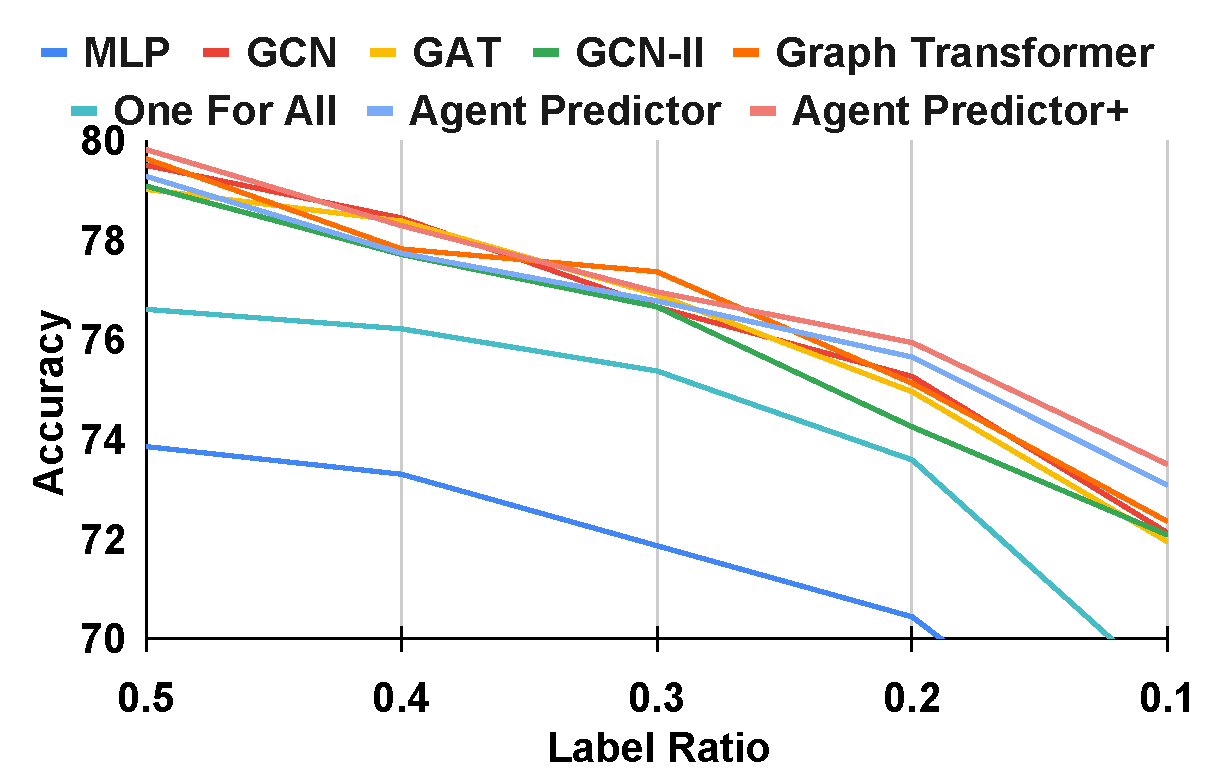
\includegraphics[width=0.355\textwidth]{figures/label_ratio.pdf}
    \vspace*{-0.5cm}    
    \caption{Accuracy comparison between \ours{} and the baselines across varying label ratios.} \label{figure:label_ratio}
    \vspace*{-0.2cm}
\end{wrapfigure}

\textbf{Effects of Pretraining Phase (Q3)}. Since acquiring a large amount of ground-truth labels from agentic workflows is expensive, we examine whether cross-domain unsupervised pretraining (denoted as \ours{}+) benefits settings where labeled instances are limited. We vary the label ratio from 0.1 to 0.5, selecting labeled samples from the training split of all datasets in the benchmark. We pretrain the proposed multi-view encoder on the remaining 50\%\,($M$) of the training set with a batch size of 32 for 20 epochs. See more details in \S\ref{section:full_pretrain}. On average, the results shown in \autoref{figure:label_ratio} indicate that \ours{}+ consistently outperforms all baseline models across all label ratios, demonstrating the effectiveness of our unsupervised pretraining strategy. The gains are especially pronounced in low-label regimes: at a 0.1 label ratio, \ours{}+ maintains an accuracy above 73\%, while other models drop closer to 70\%. These findings underscore the importance of leveraging cross-domain structure through pretraining for generalizable workflow performance prediction, especially when direct supervision is limited.


\textbf{Out-of-Distribution (OOD) Performance (Q4)}. We evaluate OOD robustness under \emph{cross-system} generalization (training on one agentic framework and testing on another) and \emph{cross-domain} generalization (training on one task domain and testing on disjoint domains). As shown in \S\ref{section:ood_results}, \ours{} consistently generalizes beyond in-distribution memorization, maintaining strong performance and preserving relative workflow rankings across both settings. For example, when trained on AFlow and tested on G-Designer, \ours{} improves average accuracy from 59.52\% (best baseline) to 62.05\% and utility from 55.33\% to 58.49\%. Similar gains hold in the reverse direction and under cross-domain splits.


\textbf{Comparison with LLM Predictors (Q5)}. We evaluate 5-shot, prompt-based LLM classifiers\,(temperature 0) using the standardized LLM-PP template\,\citep{LLM_PP} with GPT-4.1, Claude 4 Sonnet, and Gemini 2.5 Flash. As shown in \autoref{table:llm_fewshot_results}, these prompt-only LLM predictors substantially underperform our graph-based model, indicating that they struggle to exploit the structured nature of agentic workflows. \ours{} achieves 84.97\% accuracy and 81.37\% utility, far exceeding the second-best GPT-4.1 at 62.86\% and 58.92\%, while also avoiding the considerable latency and monetary overhead of LLM inference. Overall, few-shot LLMs serve as a useful baseline but remain less effective and less economical for large-scale agent search.



\subsection{Resource Cost} \label{section:cost_analysis}

\begin{wraptable}{r}{0.4\textwidth}
\vspace*{-0.75cm}
\caption{Computation cost comparison.} \label{table:cost_analysis}
\resizebox{0.4\textwidth}{!}{%
\begin{tabular}{@{}c|cc|cc@{}}
\toprule
\multirow{2}{*}{\textbf{Model}} & \multicolumn{2}{|c}{\textbf{Training}} & \multicolumn{2}{|c}{\textbf{Inference}} \\ \cmidrule(l){2-5} 
 & \textbf{Time (s/epoch)} & \textbf{Memory (GB)} & \textbf{Time (ms/sample)} & \textbf{Memory (GB)} \\ \midrule \midrule
MLP & 0.195 & 0.033 & 0.002 & 0.020 \\ \midrule 
GCN & 4.867 & 0.058 & 0.017 & 0.040 \\
GAT & 5.108 & 0.058 & 0.023 & 0.042 \\
GCN-II & 4.623 & 0.058 & 0.015 & 0.040 \\
Graph Transformer & 5.372 & 0.087 & 0.023 & 0.060 \\
Dir-GNN & 4.965 & 0.077 & 0.023 & 0.050 \\
One For All & 6.140 & 0.038 & 0.018 & 0.038 \\ \midrule
GPT-4.1 & \multicolumn{2}{c|}{\multirow{3}{*}{\begin{tabular}[|c]{@{}c@{}}N/A\\ (via OpenRouter API)\end{tabular}}} & 2253.333 & \multirow{3}{*}{N/A} \\
Claude 4 Sonnet & \multicolumn{2}{c|}{} & 1888.333 &  \\
Gemini 2.5 Flash & \multicolumn{2}{c|}{} & 2606.667 &  \\ \midrule
\begin{tabular}[c]{@{}c@{}}\emph{\ours{}}\\ (+ pretraining)\end{tabular} & \begin{tabular}[c]{@{}c@{}}4.840\\ (168.104)\end{tabular} & \begin{tabular}[c]{@{}c@{}}2.760\\ (13.520)\end{tabular} & 0.054 & 0.490 \\ 
\bottomrule
\end{tabular}%
}
\vspace*{-0.3cm}
\end{wraptable}


We further examine the efficiency of \ours{} measured by computation time and memory usage. As shown in \autoref{table:cost_analysis}, our framework remains competitive with standard GNN baselines despite its higher model capacity and richer input features, requiring only 0.054ms and 0.49GB to score a workflow at inference---orders of magnitude faster and cheaper than few-shot LLM predictors. A full run of \ours{} involves a one-time cost of $\approx1.2$ A100 GPU-hours\,(200 supervised epochs plus 20 optional pretraining epochs), with modest memory requirements that fit on a single 16 GB GPU. In contrast, LLM-based scoring costs about \$21 per 1,000 candidates ($\approx$\$0.021 per sample with Gemini 2.5 Flash), implying a break-even point after only 110-120 evaluations assuming a \$2/hr A100 rate. As realistic searches involve thousands of candidates and the trained predictor is reusable across tasks and frameworks, this modest one-time cost is quickly amortized, making \ours{} far more economical than repeated LLM calls while offering near-zero marginal latency and higher accuracy.




Full experimental results on different underlying LLMs, various GNN backbones, LLM classifier comparison, and out-of-distribution test are reported in Tables~\ref{table:llm_backbones} \ref{table:gnn_backbones}, \ref{table:llm_fewshot_results}, \ref{table:ood_aflow}, \ref{table:ood_gd} and \ref{table:cross_domain}, respectively. An additional evaluation of performance predictors used as a reward function for agentic workflow optimization, and case study findings are also provided in \S\ref{section:workflow_results} and \S\ref{section:case_study}.


